\documentclass{beamer}

% \documentclass[handout]{beamer}   % Crea slide per la stampa
% \setbeameroption{show notes on second screen=right} % Both screen option

\usepackage[italian]{babel}
\usepackage[utf8]{inputenc}
\usepackage[T1]{fontenc}
\usepackage{graphicx} % Per inserire immagini
\usepackage{booktabs} % Pacchetto per tabelle
\usepackage{caption}  % Per didascalie
\usepackage{microtype} % Migliora la tipografia

% Impostazioni tema
\usetheme{Madrid} % Tema delle slide
\useinnertheme{rectangles}
\setbeamertemplate{blocks}[default]

% \useoutertheme[right]{sidebar} % Barra laterale (facoltativo)
\usefonttheme{serif}

% Gestione bibliografia con biblatex
\usepackage[backend=bibtex]{biblatex}
\bibliography{bibliografia}

\usepackage{anyfontsize} % Per evitare errore fontsize

\usepackage{hyperref}
\hypersetup{
    pdfauthor={Alan Leoni, alan.leoni@edu.ti.ch},
    pdfnewwindow=true,
    colorlinks=false,
    linkcolor=blue,
    filecolor=blue,
    urlcolor=blue,
    citecolor=blue
}

% Definizione colori (non è necessario caricare di nuovo xcolor)
\definecolor{commentGray}{rgb}{0.3, 0.3, 0.3}
\definecolor{editorGray}{rgb}{0.95, 0.95, 0.95}
\definecolor{editorOcher}{rgb}{1, 0.5, 0}
\definecolor{editorGreen}{rgb}{0, 0.5, 0}
\definecolor{editorRed}{rgb}{0.8, 0, 0}
\definecolor{tableGray}{rgb}{0.9, 0.9, 0.9}

% Rinomina Listings to ...
\AtBeginDocument{
    \renewcommand{\lstlistingname}{Codice} % Listing -> Codice
    \renewcommand{\lstlistlistingname}{List of \lstlistingname s} % List of Listings -> List of Codici
}

\usepackage{listings}
\lstset{
  backgroundcolor=\color{editorGray},
  basicstyle={\small\ttfamily},
  frame=l,
  xleftmargin={0.75cm},
  numbers=left,
  stepnumber=1,
  firstnumber=1,
  numberfirstline=true,
  keywordstyle=\color{editorRed}\bfseries,
  commentstyle=\color{commentGray}\ttfamily,
  ndkeywordstyle=\color{editorGreen}\bfseries,
  stringstyle=\color{editorOcher},
  alsodigit={.:;},
  tabsize=2,
  showtabs=false,
  showspaces=false,
  showstringspaces=false,
  extendedchars=true,
  breaklines=true
}

% Slide con il nome della sezione
\AtBeginSection[]{
  \begin{frame}
  \vfill
  \centering
  \begin{beamercolorbox}[sep=8pt,center,shadow=true,rounded=true]{title}
    \usebeamerfont{title}\insertsectionhead\par%
  \end{beamercolorbox}
  \vfill
  \end{frame}
}

% Definizione variabili
\newcommand{\docente}{ASPE 1CD}
\newcommand{\titolo}{Presa di appunti}
\newcommand{\sottotitolo}{Applicativo OneNote}
\newcommand{\sottotitoloSmall}{}
\newcommand{\istituto}{Scuola cantonale di commercio Bellinzona}
\newcommand{\istitutoSmall}{Scc Bellinzona}
\newcommand{\materia}{Area di sperimentazione}
\newcommand{\classe}{Classe prima}
\newcommand{\email}{\texttt{}}

%%%%%%%%%%%%%%%%%%%%%%%%%%%%%%%%%%%%%%%%%%%%%%%%%%%%%%%%%%%%%%%%%%%%%%%%%
% PRIMA SLIDE
\title[\sottotitoloSmall]{\titolo}
\subtitle{\sottotitolo}
\author[\docente]{\docente\\\email}
\institute[\istitutoSmall]{\istituto\\\materia\\\classe}
\date{}

\setbeamercovered{dynamic} % (semi)trasparenza per elementi che appaiono successivamente

\begin{document}

% Crea la prima slide con il titolo
\begin{frame}
\maketitle
\thispagestyle{empty}
\end{frame}

% Crea il sommario dei contenuti
\begin{frame}
  \frametitle{Sommario}
  \tableofcontents
\end{frame}

\section{Presa di appunti durante ASPE}
\begin{frame}
  \frametitle{Perché prendere appunti?}

  \begin{itemize}
    \item Simuliamo un ambiente aziendale: le attività e le decisioni prese sono importanti
    \item Gli appunti aiutano a:
      \begin{itemize}
        \item Tenere traccia delle attività svolte
        \item Memorizzare processi e decisioni
      \end{itemize}
  \end{itemize}
\end{frame}

\begin{frame}
  \frametitle{Benefici della presa di appunti}

  \begin{itemize}
    \item Rivedere gli appunti consente di:
      \begin{itemize}
        \item Analizzare eventuali errori
        \item Migliorare le strategie simulate
      \end{itemize}
    \item Organizzare il proprio lavoro in modo più strutturato
    \item Prepararsi meglio per i momenti formativi
  \end{itemize}
\end{frame}

\begin{frame}
  \frametitle{Riflessione sugli appunti}

  \begin{itemize}
    \item Non basta scrivere, è necessario riflettere su quanto fatto:
      \begin{itemize}
      \item Quali decisioni sono state giuste?
      \item Quali quelle poco efficaci?
      \item Dove è possibile migliorare?
      \end{itemize}
    \item La riflessione rafforza la comprensione e stimola il miglioramento continuo
  \end{itemize}
\end{frame}

\begin{frame}
  \frametitle{Un esempio concreto}
  \framesubtitle{Una decisione aziendale}
  \begin{block}{Scenario}
    La mia isola ha simulato la creazione di una campagna di marketing per un nuovo prodotto
  \end{block}
\end{frame}

\begin{frame}
  \frametitle{Un esempio concreto}
  \framesubtitle{Una decisione aziendale}
  Spunti di riflessione per la presa di appunti:
      \begin{itemize}
        \item Quali canali di marketing sono stati scelti e perché
        \item I costi stimati e i tempi di realizzazione della campagna
        \item Quali sfide sono emerse durante il processo e come sono state affrontate
      \end{itemize}
\end{frame}

\begin{frame}
  \frametitle{Un esempio concreto}
  \framesubtitle{Una decisione aziendale}
  Riflettendo su questi appunti, si può analizzare:
  \begin{itemize}
  \item Se la scelta dei canali è stata efficace
  \item Come migliorare la gestione delle sfide in future simulazioni
  \end{itemize}
\end{frame}

\section{Microsoft OneNote}

\begin{frame}
  \frametitle{Cos'è OneNote?}

  \begin{itemize}
    \item OneNote è un blocco appunti digitale
    \item Permette di organizzare gli appunti in sezioni e pagine
    \item Strumento versatile per prendere, organizzare e \texttt{condividere} appunti
  \end{itemize}
\end{frame}

\begin{frame}
  \frametitle{OneNote}
  \begin{center}
    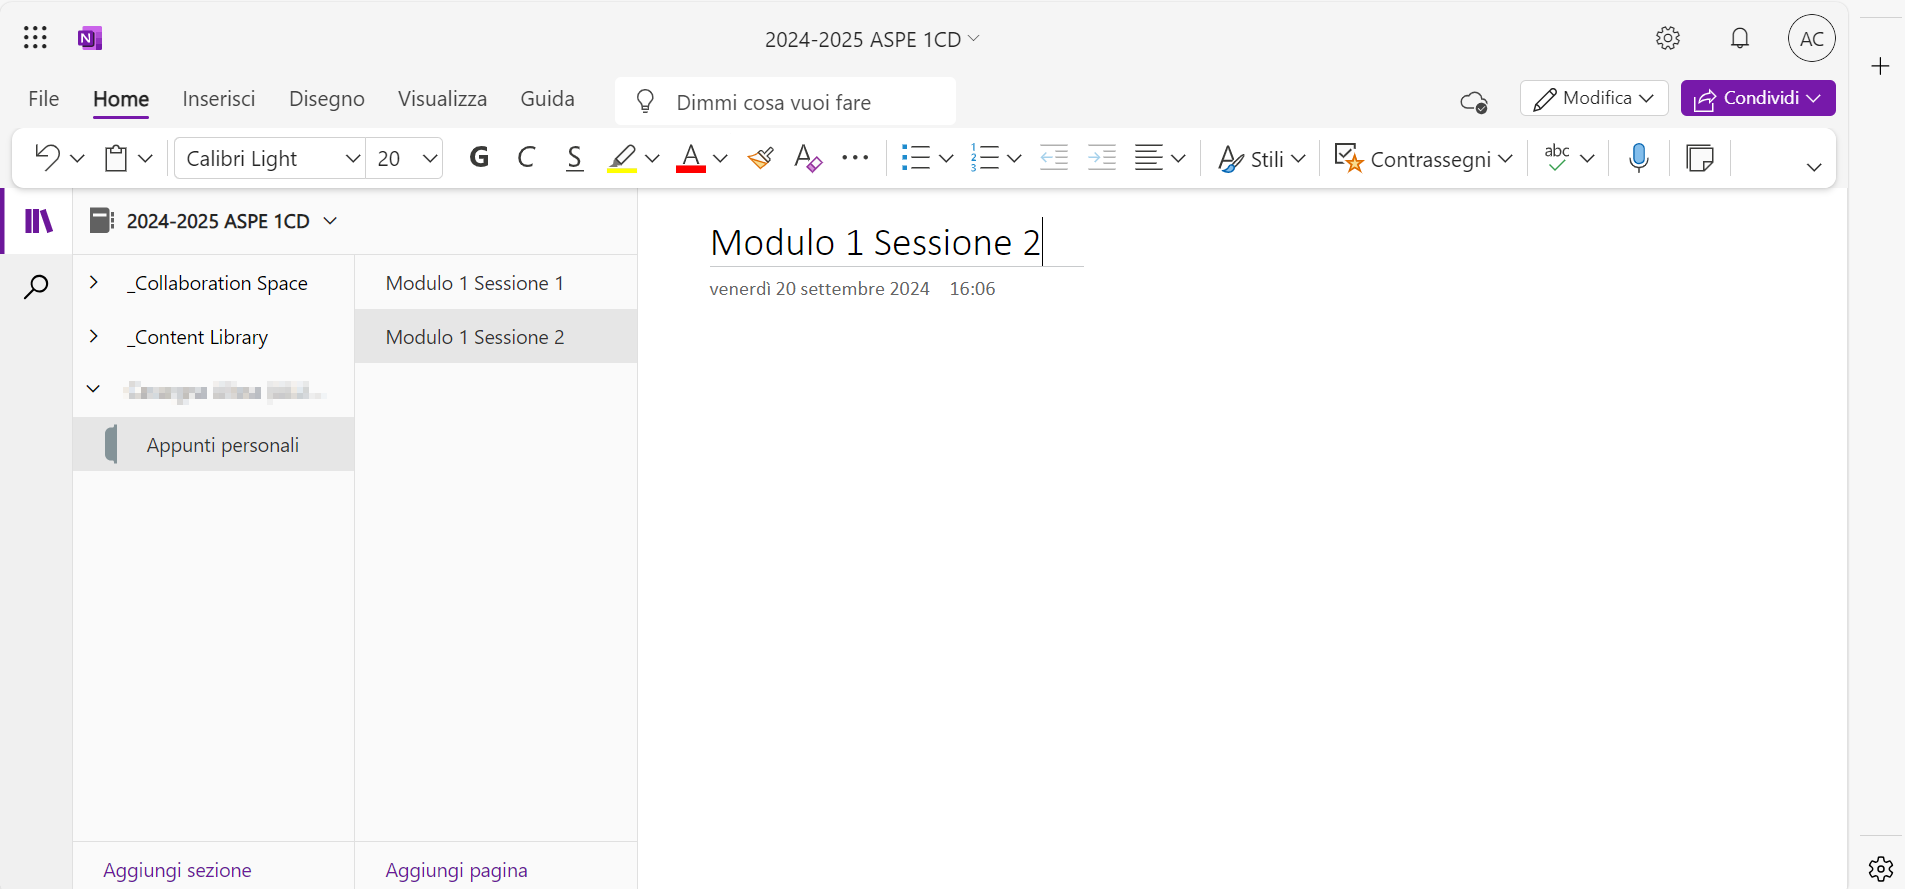
\includegraphics[width=0.9\linewidth]{images/7.png}
  \end{center}
\end{frame}


\begin{frame}
  \frametitle{Caratteristiche principali di OneNote}

  \begin{itemize}
    \item \textbf{Sezioni}: utilizzate per suddividere gli argomenti o le aree di lavoro
    \item \textbf{Pagine}: all'interno delle sezioni, si organizzano i dettagli specifici (una pagina per \texttt{sessione})
    \item Facile inserimento di testo, immagini e allegati per arricchire i contenuti
    \item Accessibile da diversi dispositivi (sia a scuola che da casa)
  \end{itemize}
\end{frame}

\begin{frame}
  \frametitle{Utilizzo di OneNote nel corso}

  \begin{itemize}
    \item Ogni studente avrà accesso a un blocco appunti condiviso esclusivamente con i docenti
    \item Le pagine saranno così organizzate:
      \begin{itemize}
        \item Attività aziendali simulate
        \item Riflessioni personali
      \end{itemize}
  \end{itemize}
\end{frame}

\section{Primo accesso a OneNote}
\begin{frame}
  \frametitle{Requisiti}
  \begin{itemize}
  \item Avere accesso al proprio networkID (es. ybn750@edu.ti.ch)
  \item Conoscere il link di accesso: \texttt{fornito dal docente}
  \end{itemize}
\end{frame}
\note{
  \begin{itemize}
  \item Link classe 1CD 2024-2025
  \item \url{https://www.onenote.com/classnotebook/view?NotebookUrl=https%3A%2F%2Fedutich-my.sharepoint.com%2Fpersonal%2Fybn750_edu_ti_ch%2FDocuments%2FClass%2520Notebooks%2F2024-2025%2520ASPE%25201CD
}
  \end{itemize}
}

\begin{frame}
  \frametitle{Primo accesso}
  \begin{center}
    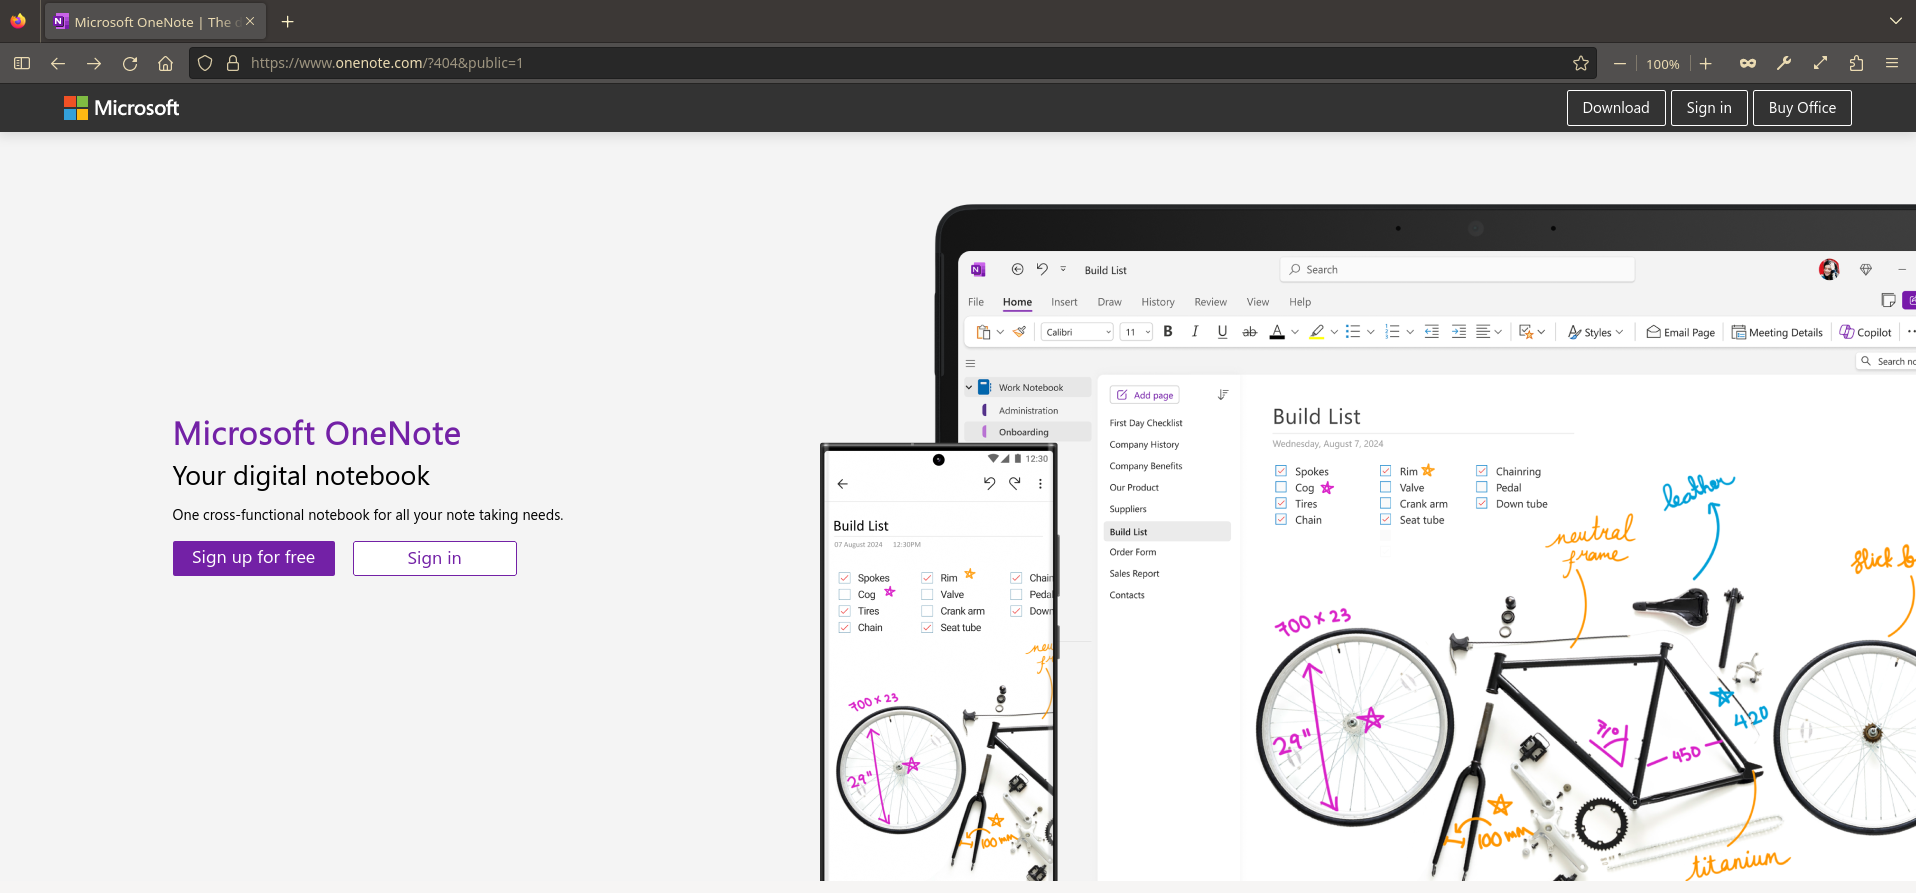
\includegraphics[width=0.8\linewidth]{images/1.png}
  \end{center}
\end{frame}

\begin{frame}
  \frametitle{Primo accesso}
  \begin{center}
    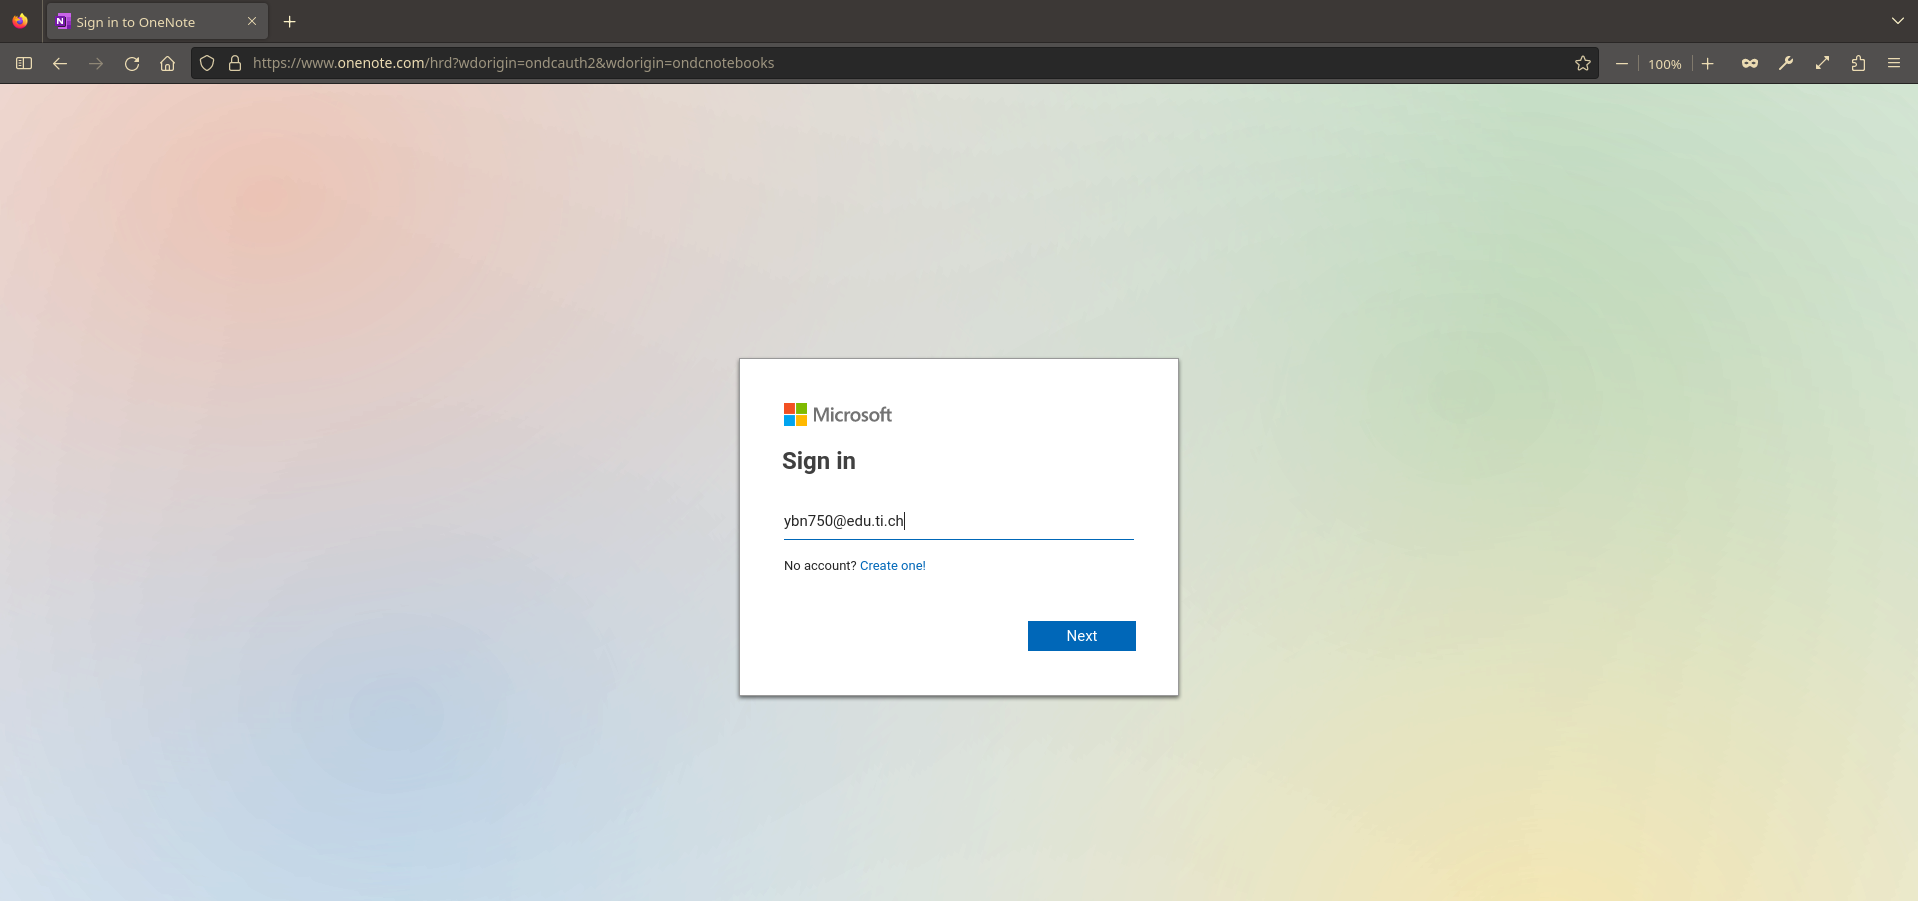
\includegraphics[width=0.8\linewidth]{images/2.png}
  \end{center}
\end{frame}

\begin{frame}
  \frametitle{Primo accesso}
  \begin{center}
    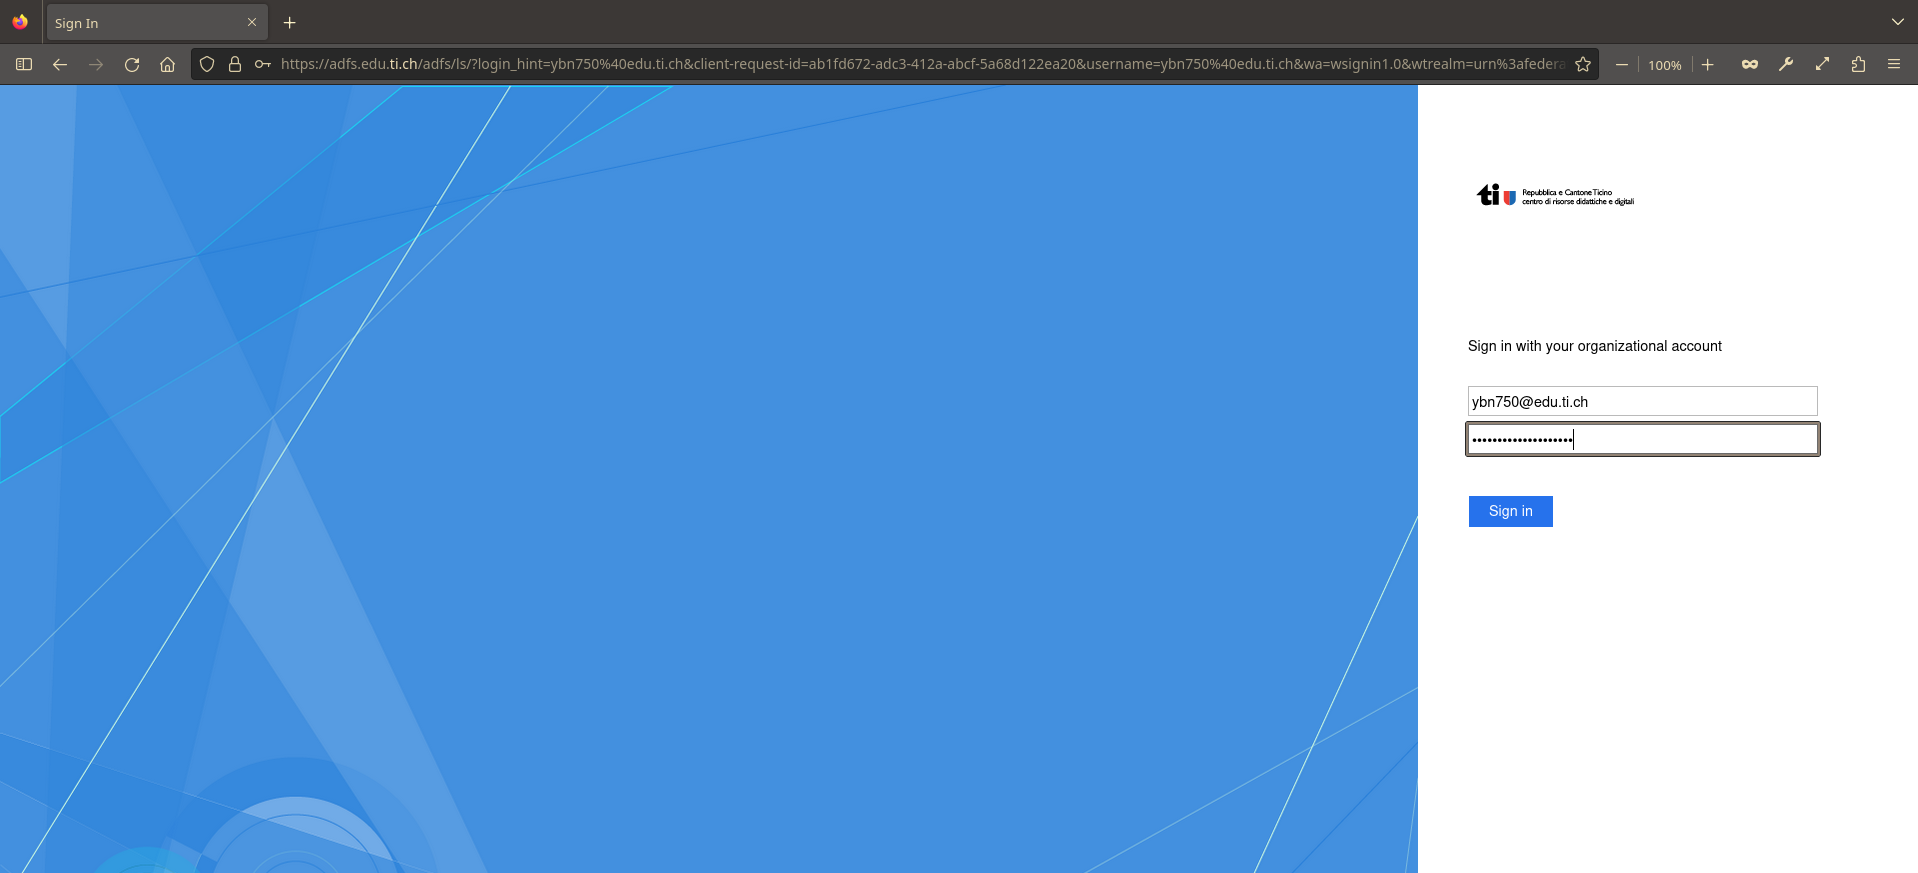
\includegraphics[width=0.8\linewidth]{images/3.png}
  \end{center}
\end{frame}

\begin{frame}
  \frametitle{Primo accesso}
  \begin{center}
    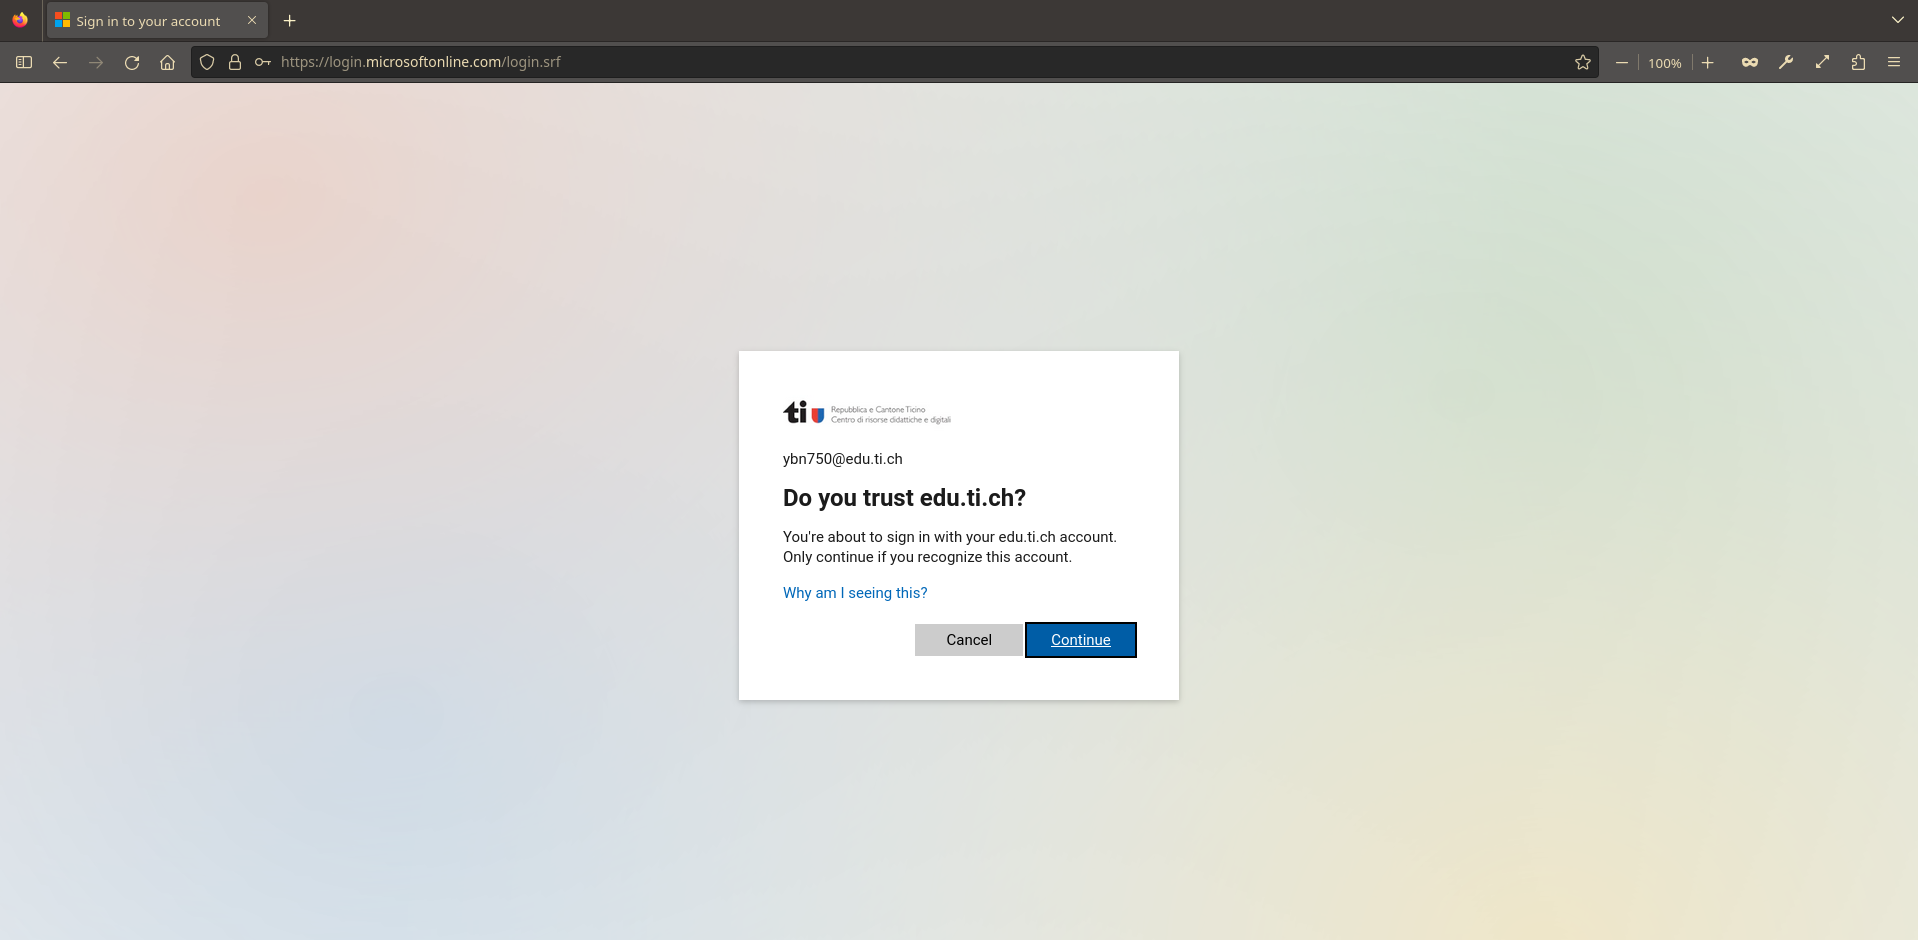
\includegraphics[width=0.8\linewidth]{images/4.png}
  \end{center}
\end{frame}

\begin{frame}
  \frametitle{Primo accesso}
  \begin{center}
    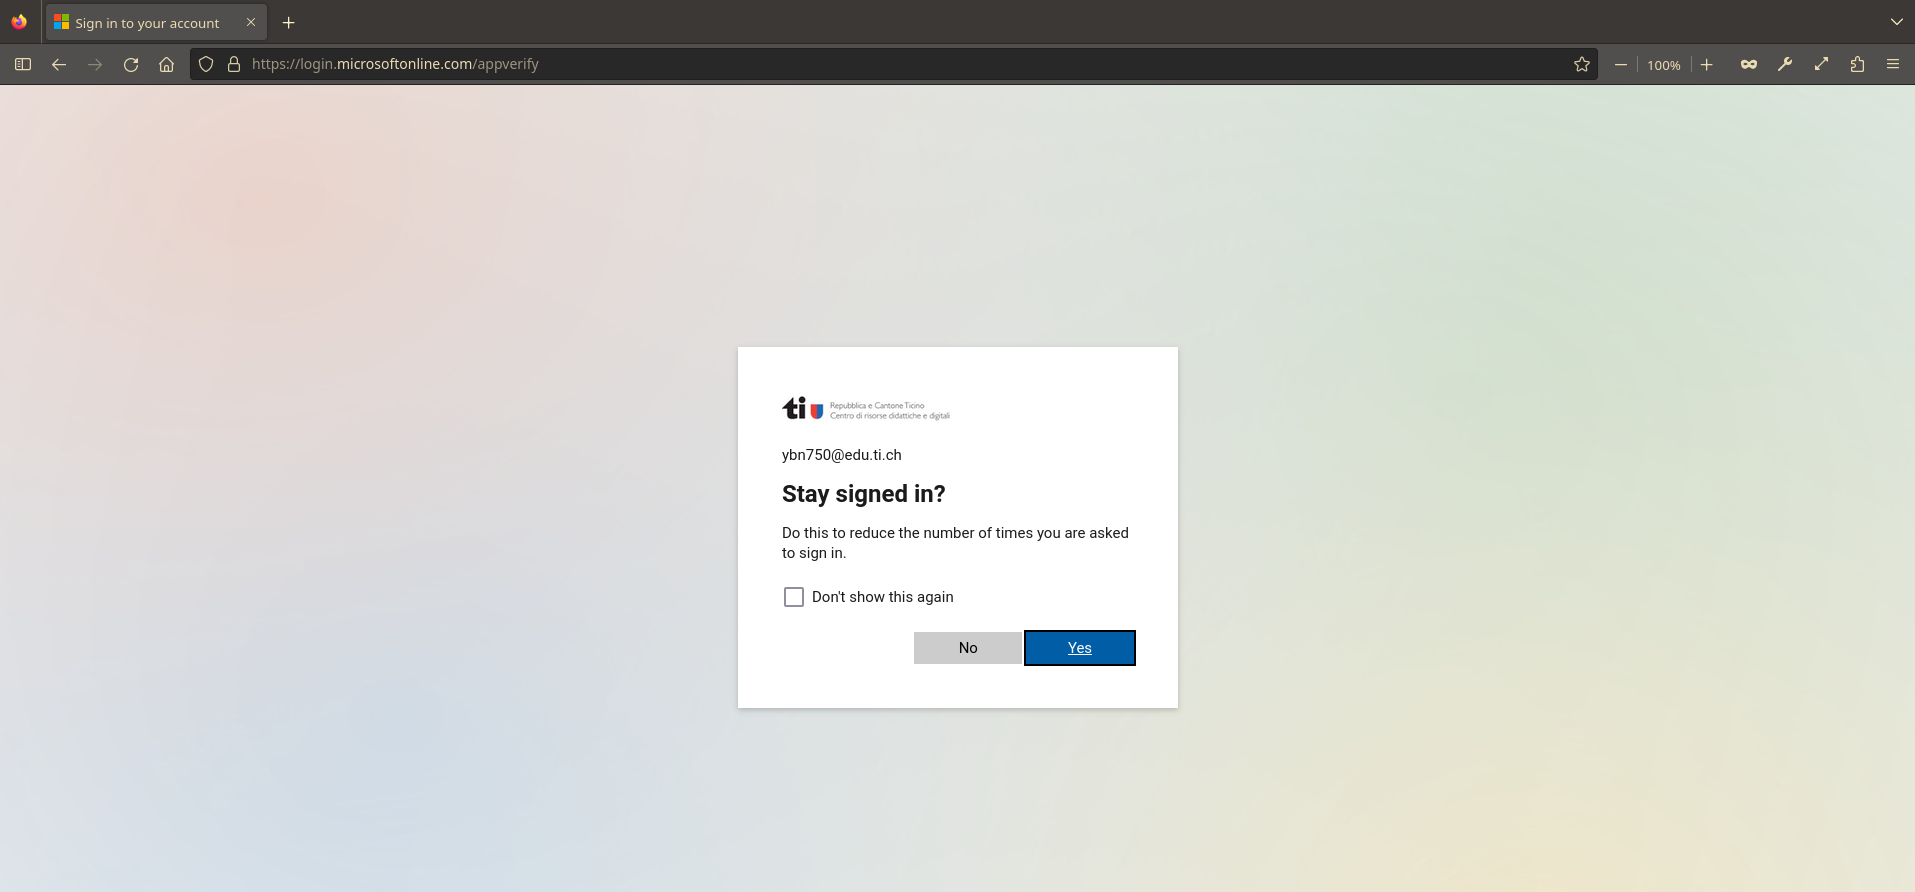
\includegraphics[width=0.8\linewidth]{images/5.png}
  \end{center}
\end{frame}

\begin{frame}
  \frametitle{Primo accesso}
  \begin{center}
    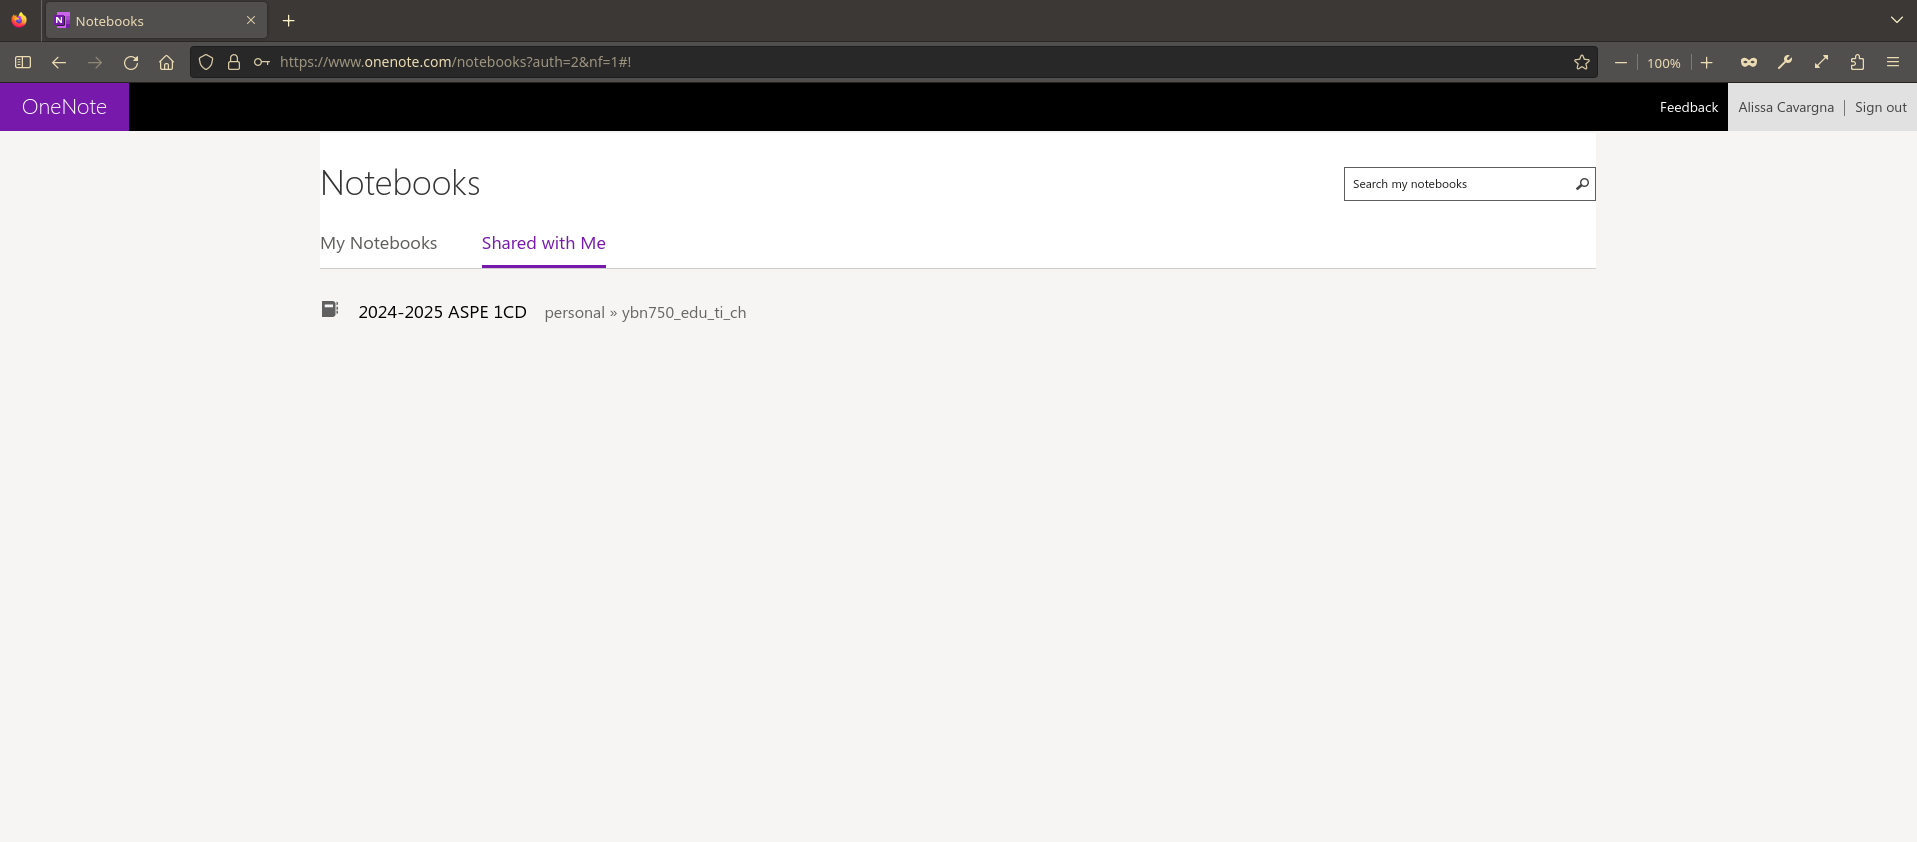
\includegraphics[width=0.8\linewidth]{images/6.png}
  \end{center}
\end{frame}

\begin{frame}
  \frametitle{Primo accesso}
  \begin{center}
    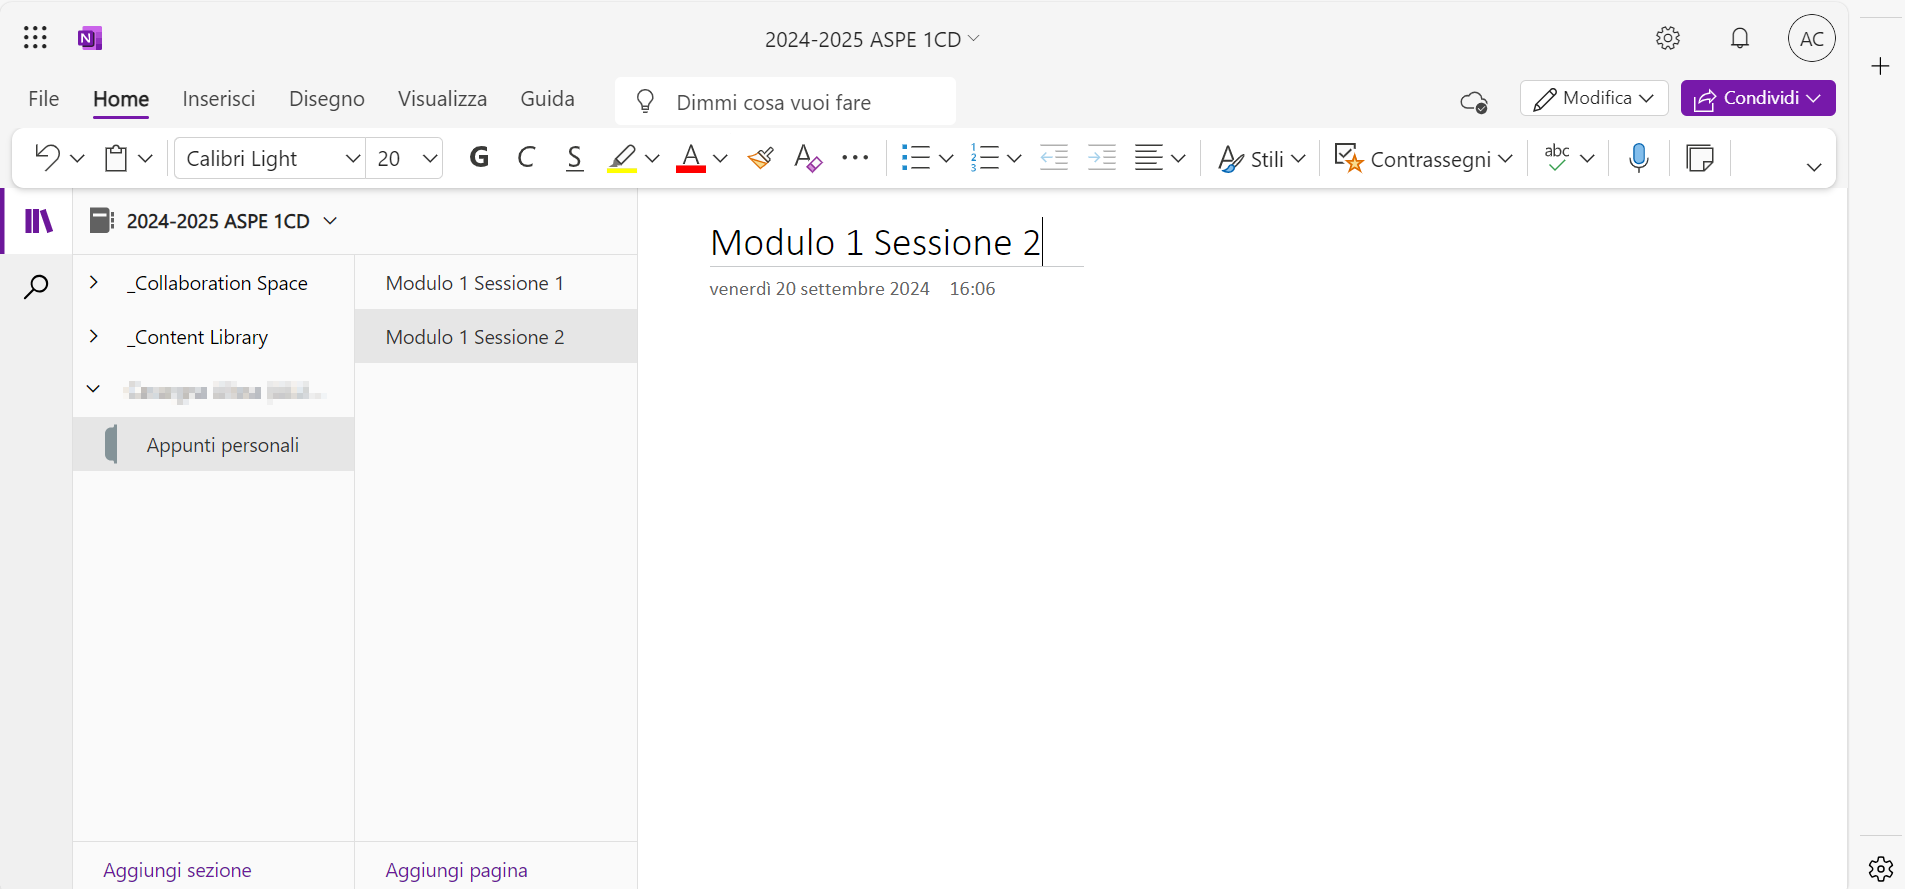
\includegraphics[width=0.8\linewidth]{images/7.png}
  \end{center}
\end{frame}

\section{Accessi successivi}  
\begin{frame}
  \frametitle{Accessi successivi}
  \begin{itemize}
  \item \url{https://office.com}
  \item Credenziali di accesso: \textit{networkID}
  \end{itemize}
\end{frame}

\begin{frame}
  \frametitle{Accessi successivi}
  \begin{center}
    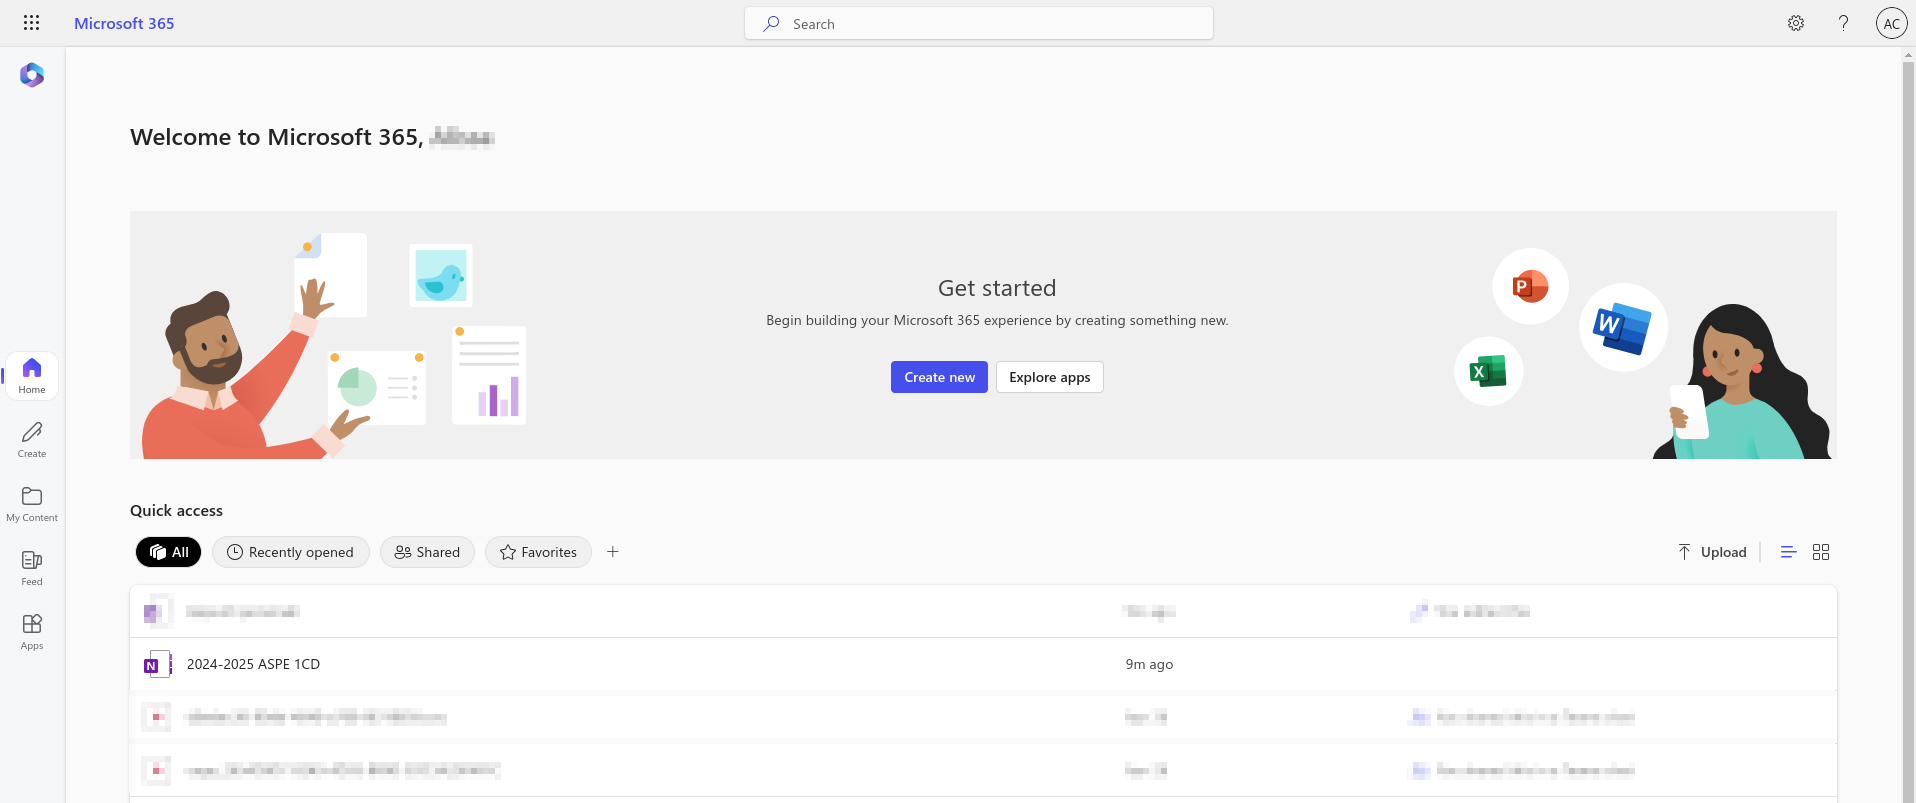
\includegraphics[width=0.8\linewidth]{images/8.png}
  \end{center}
\end{frame}

\begin{frame}
  \frametitle{Accessi successivi}
  \begin{center}
    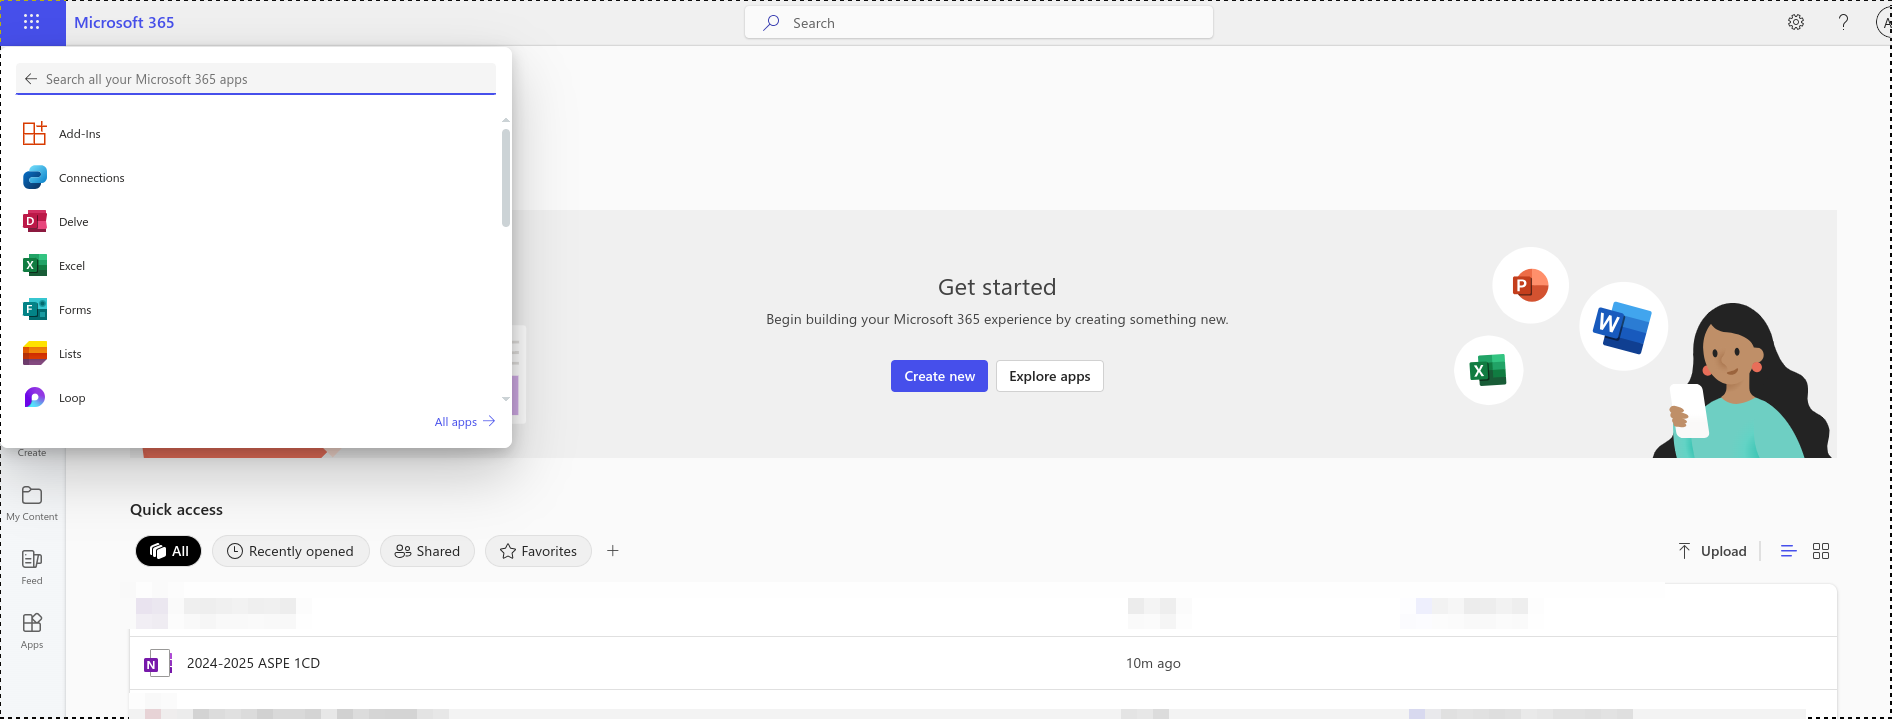
\includegraphics[width=0.8\linewidth]{images/9.png}
  \end{center}
\end{frame}

\begin{frame}
  \frametitle{Accessi successivi}
  \begin{center}
    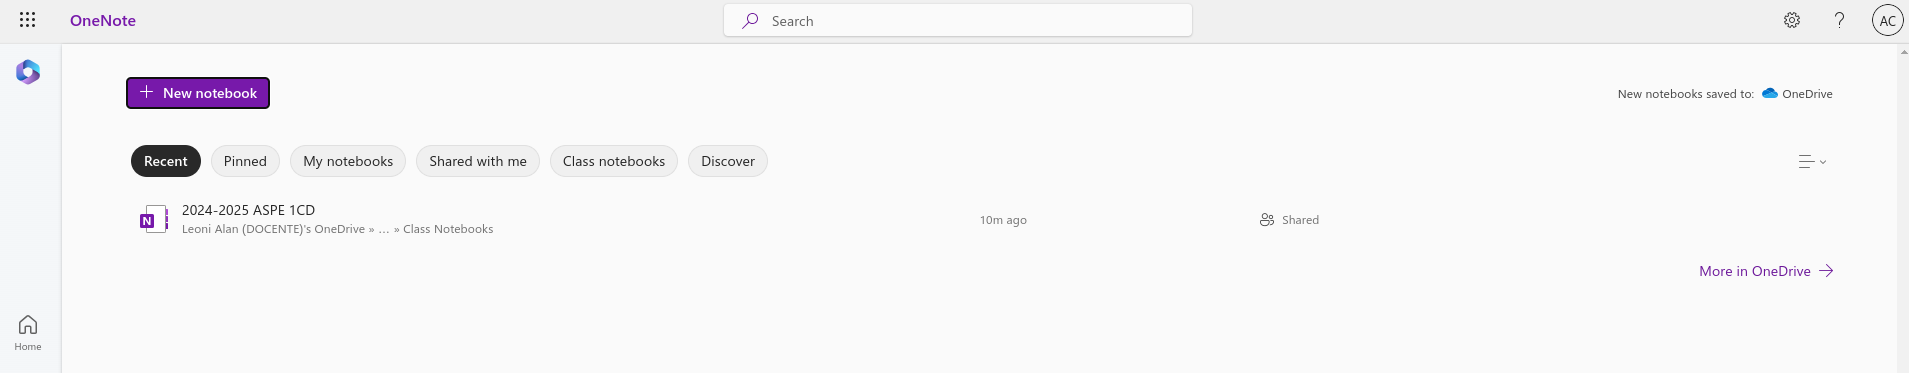
\includegraphics[width=0.8\linewidth]{images/10.png}
  \end{center}
\end{frame}


%%%%%%%%%%%%%%%%%%%%%%%%%%%%%%%%%%%%%%%%%%%%%%%%%%%%%%%%%%%%%%%%%%%%%%%%% 
% % Riferimenti bibliografici
% \begin{frame}[allowframebreaks, noframenumbering]
%   \frametitle{Riferimenti immagini}
%   \printbibliography[type=online]
% \end{frame}

% \begin{frame}[allowframebreaks, noframenumbering]
%   \frametitle{Riferimenti bibliografici}
%   \printbibliography[type=article]
%   \printbibliography[type=book]
% \end{frame}

%%%%%%%%%%%%%%%%%%%%%%%%%%%%%%%%%%%%%%%%%%%%%%%%%%%%%%%%%%%%%%%%%%%%%%%%%
% % Licenza
% \begin{frame}
%   \frametitle{Licenza}
%   \centering
%   ©\docente
%   \begin{figure}[h]
%     
\includegraphics[width=0.4\textwidth]{images/cc}
%   \end{figure}
%   Tranne che dove menzionato diversamente, questo lavoro è
%   distribuito sotto licenza Creative Commons
%   Attribution-NonCommercial-NoDerivatives 4.0 International License.\\
%   Per avere una copia di questa licenza, visitare:
%   \url{https://creativecommons.org/licenses/by-nc-nd/4.0/}.
% \end{frame}
%%%%%%%%%%%%%%%%%%%%%%%%%%%%%%%%%%%%%%%%%%%%%%%%%%%%%%%%%%%%%%%%%%%%%%%%%
\end{document}
